\section{Findings}\label{sec-findings}
\subsection{Cross-Cultural Collaboration Outcomes and Facing \&	Overcoming Challenges}\label{sub-sec-crosscultural}
	
In both years of the project, each of the respective US and Brazil PST
classes experienced similar outcomes and challenges during their
collaborations in the projects (seven weeks in 2022; and eight weeks in
2023). Some of the challenges faced in 2022 were addressed and tasks
were adjusted in the second year of the VE project (2023) to reflect the
professor’s and PSTs’ expectations and analysis of the 2022 PST's experiences. The accommodations in project design from the 2022 year while did not benefit those PSTs since that
class ended, did benefit those who participated in the 2023 VE. For
example, the PSTs from the 2022 group stated that they wanted to have
more time to get to know each other (not only to develop the assigned
tasks from the cross-cultural project). So, the professors added, in the
initial phase of the 2023 interactions, a Padlet activity for the PSTs
to get acquainted more informally, but still asynchronous to accommodate
the format of the US course.

Even in the second year, 2023 of the study with the second group of
PSTs, some issues remained as challenges. PSTs from both Brazil and the
US shared that similar to other studies, the following were challenges
to VE collaborations: coordinating their busy schedules, the
asynchronous online format (of the US course), and negotiating time zone
differences to find time for interaction and development of their
projects as many of them work and study \cite{fuchs2017multiple,evaluate2019evaluating,kern_learning_2018}.

Overcoming those challenges and important outcomes were also identified
\Cref{fig-01}:

\begin{itemize}
\item	interactional skills, such as leadership, initiative, autonomy, and collabora-tion;
\item	the development of Information and Communication Technology - ICT \cite{calvo2023investigating} and Intercultural Communicative Competence - ICC \cite{idris2019intercultural,lopez2017developing};
\item	content, cultural, and contextual knowledge;
\item	language issues.
\end{itemize}
	
In the \Cref{fig-01}, there is a representation of the outcomes and
challenges of the VE Project.
	
	
\begin{figure}[!htpb]
\centering
%Seria útil pedir a imagem em qualidade melhor, de preferência no foramto PDF.
\begin{minipage}{0.6\textwidth}
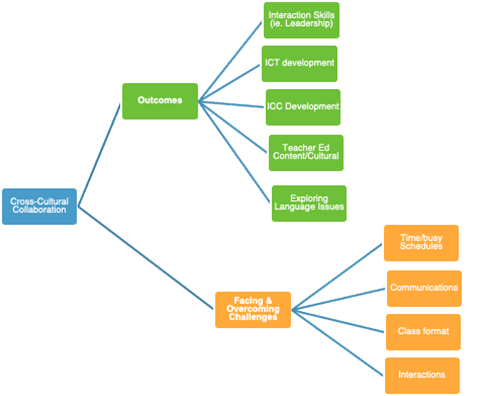
\includegraphics[width=\textwidth]{figure01.png}
\caption{Cross-Cultural Collaboration Outcomes - Facing \& Overcoming Challenges.}
\label{fig-01}
\source{Own elaboration.}
\end{minipage}
\end{figure}


\subsection{Outcomes}\label{sub-sec-outcomes}
\subsubsection{Interactional Skills}\label{sub-sub-sec-interactional}

Participating in a VE Project is a way to develop many attitudes and
skills that place the students in the center of their learning process,
as they are the ones who need to take the initiative, leadership and
autonomy for developing the tasks and collaborations. There is a \enquote{truly
learner-centered pedagogy} and it results in \enquote{increased
student-teacher responsibility} \cite{sadler2016twelve}.
		
In the analysis, it was possible to notice that some teams readily took
the initiative and appreciated the skills learned from the process. The
quote below shows how this group of students worked together to develop
the project: even being physically distant to each other, the digital
platforms enabled connection, sharing of ideas and responsibilities on
the tasks.

\begin{quote}
An initial expectation that I had was that we, as a group, would
communicate on a regular basis and have some sort of plan to dive up
responsibilities so that it would be easier for us to work on our
project. These expectations were absolutely met. We were in constant
contact, and did an excellent job or dividing all of the parts of the
presentation up. (US 2023 ST3-42)
\end{quote}

Collaboration was another aspect shared in most of the
PSTs' answers in the survey. They valued the
interaction they had with students from another part of the world; the
group work itself and the way they shared their responsibilities for
developing the project. This is probably because of the own nature of VE
projects that enable a more student-centered approach. In addition, the
professors' balance of guidance and autonomy in conducting the project
contributed to this collaborative environment.

\begin{quote}
One benefit from this was learning to be more self-dependent and
taking the instructions and collaborating with each other to put the
pieces together (US 2022 ST3-8).
	
My initial expectations for participating was that everyone will
add their input in the project and communicate with one another. These
expectations were met way beyond my expectations because everyone was on
Whatsapp chatting with each other and schedule times to communicate with
everyone with the project and everyone added their parts of the project.
(BR 2023 ST3-41)
\end{quote}

Data also indicated that some teams worked well together. Collaboration
was both a positive outcome as well as a challenge they faced and had to
overcome by applying different negotiation strategies. Some PSTs
reported collaboration in different platforms; shared
responsibilities for the project and the creative element when preparing
together the presentations. Their experiences with
telecollaboration were mixed regarding the ways they felt close or
physically distant to their colleagues. Their answers also pointed out
that they thought about their future roles as teachers when negotiating
actions and working collaboratively with other colleagues, for example:

\begin{quote}
There is something that is a benefit and a challenge at the same time, that I think that helps me becoming a better teacher, which is working in group. Me as a teacher need to know how to choose the best words to interact and make people comfortable to participate and give their opinion. I tried to do that when talking with my partners about the project, I tried to tell my opinion without being rude and being supportive. (BR 2023 ST2-58)
			
A benefit I got from this project is I learned the process of working with other educators. In my future career for example, I can use what I learned from this when working with coworkers to plan/research a unit. (US 2023 ST5-47)
\end{quote}

These quotes demonstrate that the VE Project was a context for
experiencing collaboration and developing some soft skills that are
important for their lives. When interacting with colleagues from
different cultural backgrounds, they learn to take leadership,
negotiate, and deal with conflicts.

According to \textcite{odowd2021virtual}, student’s
learning outcomes in different models of VE Projects across the globe
have to do with the way they feel "better prepared to communicate and
collaborate with people from different cultures". Hurdles or challenges
actually enhance participants' ability to find ways to creatively
collaborate and communicate with partners from other countries. Based on
O'Dowd's suggestion, for the two years of this VE project, professors
carefully designed tasks to push students out of their comfort zone, but
professors also carefully monitored the process and stayed in touch
daily to guide some PSTs who needed reminders or other support.
		
\subsubsection{ICT Development}\label{sub-sub-sec-ictdevelopment}

In a previous paper, the authors of this text identified both the
benefits and challenges of ICT during the VE Project. The following
benefits stood out: the critical nature of technology for the
communications; having choices of platforms; the uses of both
synchronous and asynchronous forms of technologies; opportunities to
help each or use trial and error learn new technologies; learning new
technologies that are used in each culture; getting to know other
students from other countries through ICT. On the other hand, the
challenges were related to time, access to the internet or internet
connection; getting in contact (i.e., email and not getting
response /communication) with everyone; and difficulties with specific
platforms. Though the authors emphasized that there were more benefits
than challenges; dealing with the challenges was important for the PSTs
to develop attitudes in their professional lives as well as for the
professors to consider important aspects of ICT when planning their
virtual collaborations \cite{calvo2023investigating}.

\begin{quote}
Having WhatsApp made the project go very smoothly. It was a great
asset to have in order to communicate with others across the world. I
remember discussing this project with my parents, and they told me how
lucky I was that we had phones and technology to do so, because when
they were younger, they had pen pals they would communicate with by
letters! I am very grateful to have had the technology to meet and work
with the girls in my group. (US 2023 ST3-42)

The benefits of technologies were the opportunity to be able to
communicate with people from another country, in addition to the ease of
access to information about who we worked with during the project, in
addition to easy access to learning from different contexts. One of the
difficulties was how to learn to use the voice thread, because, besides
the tutorial we had in the classroom, that platform is complex to use
and we had to do some steps that weren’t in the tutorial
to publish our presentation. (\emph{BR 2023} ST2-59)
\end{quote}

For both students, the technology itself was indispensable for the
interactions to happen. Besides valuing and recognizing its role in
recent educational practices, BR 2023 ST2-59, for example, also
mentions the difficulties with a specific platform, the VoiceThread.
This specific difficulty may have helped the PST to search, learn more
and use this platform.

\subsubsection{Intercultural Communicative Competence (ICC) Development}\label{sub-sub-sec-intercultural}

While seven weeks of collaboration could yield only limited shifts in
such ICC skills as mindfulness, cognitive flexibility, and impacts of
second language acquisition (Idris; Widyantoro, 2019; Üzüm; Akayoğlu;
Yazan, 2020), PSTs shared some memorable aspects of the cross-cultural
collaborations, such as motivation for the intercultural encounters,
sharing experiences, learning and respecting differences.

The analysis showed that students expressed motivation for interacting
and learning with each other. The exchanges allowed them to have contact
with people with different stories and life experiences. Often a first
step towards ICC is developing self-knowledge, by listening to others to
consider how we are different and similar. Direct and thoughtful
encounters with people, places, and foreign languages such as through VE
with students at other colleges are effective ways to begin to develop
ICC \cite{idris2019intercultural,lopez2017developing}, as PSTs in the
study indicated:

\begin{quote}
I could saw how important is try to have a contact with people
from other countries and cultures, because we can learning a lot sharing
experiences, and we can also learn to be more respectful in face of
differences. (BR 2022 ST1-26)

I think this project really showed us just how valuable it is to
learn from people that are different from us. There were many times when
we just had random group conversations, just discussing our lives, and
providing insight into the differences in our lives. (US 2023 ST3-42)
\end{quote}

\subsubsection{Content Learning and contextual information about the countries}\label{sub-sub-sec-content}
	
Data indicated that PSTs not only pointed out the contents they learned
during the VE, but they mentioned how they could learn them in a
cross-cultural way, comparing and analyzing them according to the
contextual information and reality of the two countries.

\textcite{odowd2021virtual} also found that cultural knowledge was
developed though VE Projects. According to him, in some situations,
students mentioned the factual information they learned about many
social aspects. In addition, students pointed out the development of
cultural awareness about diversity in a way to "avoid regarding cultures
as monolithic". Similarly, \textcite{kopish2020leveraging} found that students
in their study were learning from cultural experiences very different
from their own and what helped them was their desire and ability to
identify with new cultural partners.

\begin{quote}
One of the benefits of the project for my teacher education
process was to learn about the teacher education from different context
and the difference and similarities between both contexts. This is
really important for our formation, because there is not only one way
that is correct, it really depends of the culture and aspects that we
are inserted. (BR 2023 ST2-59)

The benefits would be that it allowed us to view English education
and ELLs from a different perspective, as these pre-service teachers are
all specifically going to be English teachers but a lot of the students
at [university] are going to be educators in a different subject,
but are still required to take courses that are necessary for teaching
ELLs. (US 2022 ST4-1)
\end{quote}
	
\subsubsection{Exploring Language Issues}\label{sub-sub-sec-exploring}

For many Brazilian PSTs, their English language skills were developed
and when interacting with PSTs from another context, they had
opportunities to experience language use situations that are different
from classroom activities. As all the Brazilian students were from the
Letras program (Language Arts undergraduate program), most of them were
fluent in their English communication as the VE tasks and interactions
were developed in this language.

The following illustrates the way this Brazilian PST was initially
worried about correctness; then mentions some other aspects that are
more relevant in communication (e.g. getting the message across;
negotiating meaning) that would be more important to consider in this
kind of interaction.

\begin{quote}
I could learn many things with my group. The communication was of
course a challenge for me, because I was afraid and worried about
texting correctly. Some days after, I stopped to worry about the grammar
of my written messages on WhatsApp. If my partners did not understand
something, I’ll text and write again. (BR 2023
ST4-66)
\end{quote}

Also, when participating in VE initiatives, participants may also
evaluate in different ways their linguistic competence, as one Brazilian
PST shared: \enquote{These projects clearly help the students to be proud and confident in their speeches}. (\emph{BR 2023 ST2-56}). In this
regard, \textcite[p. 217]{odowd2021virtual} found that different from
traditional ways of learning languages that are focused more on
accuracy, in telecollaborative opportunities students use the language
in a meaningful way.

PSTs from the US university related to other aspects of languages. For
example, they mentioned the role of languages in society such as: how
languages affect schools and other contexts, how other speakers are
fluent in English, how only fluency in English is not enough to avoid
misunderstandings, and their future work as teachers of bilingual
students.

\begin{quote}
[$\ldots$] The number of students from other countries both in my
school and in Brazil that were fluent in English surprised me. The
project just reinforced why it’s so important to be
bilingual and use one language to learn another. The other students were
using what they knew to understand our differences. The experience
exceeded that expectation. (US 2023 ST2-36)
	
It also highlighted how it can sometimes a language barrier can
pose a problem, even if both parties are fluent or almost fluent in a
language. There was a point where we set up a meeting, but because of
confusion based on our language differences, we met at different times
and missed our meeting. I think this could be translated to teaching
emerging bilingual students. It just opened my eyes to how beneficial
working with people who speak other languages can be, but also the
difficulties that remain. (US 2023 ST3-42)
\end{quote}

Participating in VE Projects are important initiatives not only to
develop language skills, but to understand and consider language use and
learning in a different perspective. In those excerpts, ST2-36
highlights the important way he sees the bilingual speaker using the two
languages to understand and make meaning of the experience. In the
second excerpt, ST3-42 calls the attention to the fact that fluency in
the language is only one aspect in communication - even being fluent in
their communication to schedule a meeting, they missed it because none
of the US or BR students paid attention to the time zone differences in
the countries. So, by this example, we can notice that communication is
more than just using words; it also has to do with negotiating meaning.

\subsection{Facing Challenges} \label{sub-sec-facing}
\subsubsection{Communication, interaction and collaboration}\label{sub-sub-sec-communication}

PSTs most often mentioned challenges were related to communication,
interaction, and collaboration. Some teams did not feel the
participation or initiative by some members met their expectations,
mostly due to the US PSTs in those teams not responding right away to
the Brazilian students' attempts to communicate and work on the
projects. This was probably due to the fact that the US students were
not used to communicating with WhatsApp as the Brazilian students were;
so, this cultural difference in terms of technological tools for
interaction had an impact in the initial phase of the project.

This difficulty in communication affected their organization to start
working on their projects. The Brazilian PSTs complained about the
\enquote{initial silence} from the US PSTs. Data indicated, though that soon
after getting in touch with each other, some groups could work well
together and share the responsibilities. While they were delayed with
initial responses to Brazilian PST's emails, ironically, several US PSTs
expressed that they wanted to have some more time for interactions, so
email was not the best way to start this cross cultural collaboration.
	
\begin{quote}
[$\ldots$] we did not have as much communication as I would have
liked or have expected. I do think it was interesting to talk to the
students and enjoyed what little conversations we did have. (US 2022
ST3-8)
		
I would say that one challenge that I had was communication. I had
some difficulties communicating with the rest of the group and I believe
that this could've been mitigated if there was more in person
communication. At least for me personally considering I am not the
greatest at seeing my emails. (US 2023 ST5-50)
\end{quote}
	
\subsubsection{Time and busy agendas}

Most PSTs found ICT solutions to work through the challenges of busy
schedules, time zone differences (2 hours difference) and communication
with everyone. They learned to adapt and use WhatsApp for group
communication, as an asynchronous platform for group activities/tasks
even if this was their first time learning the App.
	
\begin{quote}
[\ldots] getting ahold of everyone was difficult. For example,
our group member emailed us on to create a WhatsApp, and one of our
group mates didn't respond until [2wks later]\ldots. communication
was difficult, even with some of the students at [Univ.] because we
were all on different campuses with different schedules\ldots.but we
used resources like WhatsApp and google slides to help us communicate
with one another. I had never used WhatsApp before this assignment, so
learning how to use that app was beneficial in case I ever need to use
it again. At first, it was difficult to get a steady communication
source with everyone. However, we got it all figured out by the time our
presentation was due. (US 2022 ST3-2)
\end{quote}
	
Providing both required ICT and developing a well-planned and guided VE
framework \cite{gleason2021design} as well as allowing
students to choose their ICT, supported the development of ICC \cite{kolm2022international}. PST in this study showed they were developing
skills for communication through asynchronous and synchronous
technology, leadership, project management, and cultural diversity
through different forms of technology. Besides their busy agendas, the
class format of the classes in the two contexts had and impact on the
development of the activities. The next section explores this challenge
in the VE project.

\subsubsection{Class format}\label{sub-sub-sec-class}

Another factor that impacted the cross-cultural collaboration was the
class format; while Brazilian students had in-person classes, US
students had asynchronous web classes. So, the ways that professors
interacted with PSTs were also different; the US professor needed to
follow the development of the tasks and interactions by continuous
online check-in with their students, while the Brazilian professor had
classes with their students twice a week and gave those PSTs some class
meetings to develop activities for their respective cross-cultural
projects. Considering these differences, though, PSTs felt supported.
This Brazilian PST recognized the collaboration process among the
professors to organize the VE.

\begin{quote}
Professor [Brazil] has been very supportive and understandable
since we started this program, and so they always made it very clear
that they constantly wanted to check our work in progress, by giving
ideas, embracing others we had, and that they was always in contact with
Professor [US], who was nothing but receptive and empathetic. I
really appreciate the fact that \textbf{they} are really interested in
our culture, knowing so much about it, and being open to our suggestions
too. (BR 2023 ST4-65).
\end{quote}

This collaboration was also seen in the study of \textcite[p. 412]{sadler2016twelve} with their PSTs. The authors emphasize the mutual
responsibilities and VE joint planning/ development by the teachers. In
this way their students could see their collaboration and the use of
telecollaboration in their practices.

Because of this class format difference, the US professor took into
consideration the importance of additional asynchronous virtual
scaffolding and explanation about the project. Balancing the amount of
scaffolding (reminders about upcoming tasks or reminders to read their
messages from the BR PSTs, extra directions, or video/picture
directions) with supporting and encouraging students’
autonomy was at the forefront of the professors’
consideration when planning and implementing the VE tasks.




